\chapter{TINJAUAN PUSTAKA}
\label{chap:tinjauanpustaka}

\section{Hasil Penelitian Terdahulu}
\label{sec:hasilpenelitianterdahulu}
Terdapat beberapa penelitian sebelumnya yang membahas mengenai topik kontrol PowerPoint menggunakan pose tangan. Berdasarkan penelitian terdahulu ini dapat dijadikan referensi serta dicari gap apa yang dapat ditingkatkan lagi dalam penelitian ini. Berikut ini adalah beberapa penelitian terdahulu tersebut.
\subsection{\emph{Power Point Slideshow Navigation Control with Hand Gestures using Hidden Markov Model Method}}
\label{subsec:Power Point slideshow navigation control with hand gestures using Hidden Markov Model method}
Dalam penelitian dengan judul \emph{"Power Point slideshow navigation control with hand gestures using Hidden Markov Model method"}, yang ditulis oleh C. Rahmad, A. Prasetyo, dan R. A. Baqy, dibahas mengenai kontrol PPT menggunakan pose tangan juga. Namun, dalam penelitian tersebut metode yang digunakan berbeda dengan penelitian ini, yaitu \emph{Markov Model Method}. Selain itu, terdapat beberapa hal yang dapat ditingkatkan dari penelitan tersebut. Pertama adalah tingkat akurasinya diangka 76,47\% dengan jarak maksimal 150 cm. Akurasi ini diharapkan dapat lebih ditingkatkan pada penelitian ini. Hal yang dapat ditingkatkan yang kedua adalah pada penelitian ini deteksi yang dilakukan terbatas pada jarak yang sesuai dengan dataset yang diberikan. Sehingga apabila jarak antara pengguna dengan kamera tidak sesuai dengan dataset yang diberikan, akurasinya menurun secara drastis \parencite{Rahmad2022}.

\subsection{\emph{Power Point Control Using Hand Gesture
Recognition Based on Hog Feature Extraction And
K-NN Classification}}
\label{subsec:Power Point Control Using Hand Gesture
Recognition Based on Hog Feature Extraction And
K-NN Classification}
Hasil yang diusulkan dalam penelitian ini adalah membuat program yang memungkinkan manusia untuk mengontrol presentasi PowerPoint tanpa menggunakan perangkat keras apa pun di antaranya, hanya menggunakan kamera dan gestur tangan. Penelitian ini melakukan proses ekstraksi fitur \emph{Histogram-of-Gradient} dari masukan gambar dan mengklasifikasikannya kedalam salah satu dari empat
isyarat menggunakan algoritma \emph{K-NN Classification}. Terdapat empat klasifikasi yang dilakukan yaitu \emph{next slide, previous slide, go to first slide,} dan \emph{End of Presentation}. Keakuratan yang dicapai dalam penelitian ini berada pada kisaran 80\% \parencite{Tejashree2017}. 

\section{Dasar Teori}
\label{sec:dasarteori}
Dasar teori berisi berbagai teori yang memiliki keterikatan dengan penelitian yang dilakukan sebagai dasar pemahaman mengenai konsep tertentu. Berikut adalah dasar teorinya.

\subsection{Pose Tangan}

Pose menurut Kamus Besar Bahasa Indonesia (KBBI) merupakan gaya atau sikap yang ditampilkan baik ketika dipotret, digambar atau dilukis. Sedangkan tangan merupakan anggota badan dari siku sampai ke ujung jari atau dari pergelangan sampai ujung jari. Sehingga, dapat dinyatakan bahwa pose tangan merupakan gaya atau sikap yang ditampilkan bagian tubuh dari pergelangan sampai ujung jari dan kemudian dipotret untuk tujuan tertentu.

Pose tangan menjadi salah satu bentuk yang dapat digunakan untuk berinteraksi antar manusia untuk mengirimkan pesan tertentu secara efektif dan mudah dipahami. Oleh karena itu, pose tangan juga menginspirasi untuk digunakan sebagai sarana komunikasi dalam berinteraksi antara manusia dengan komputer. 

Interaksi Manusia Komputer atau lebih terkenal dengan istilah \emph{Human Computer Interaction} (HCI), bertujuan untuk meningkatkan interaksi antara pengguna dan komputer dengan membuat komputer lebih bermanfaat dan menerima yang pengguna butuhkan. Bidang ini menjadi salah satu bidang yang berkembang pesat selama beberapa tahun terakhir.

Karena pesatnya perkembangan yang terjadi pada bidang ini, akhirnya banyak variasi dan cara yang digunakan sebagai sinyal masukan. Salah satunya adalah pose tangan. Hal ini memungkinkan karena perkembangan perangkat keras seperti kamera yang semakin berkualitas. Tidak hanya itu, bagian yang terpenting dalam pekembangan bidang ini adalah adanya algoritma \emph{machine learning} yang semakin canggih untuk dapat membuat komputer memahami suatu citra yang diterima melalui input kamera. 

Pose tangan juga menjadi sarana komunikasi yang dapat menggantikan banyak perangkat keras tambahan. Mekanisme input, yang biasanya diberikan oleh \emph{mouse}, \emph{keyboard}, \emph{remote control} atau panel layar sentuh, bisa jadi diganti dengan dengan menggunakan satu perangkat keras saja yaitu kamera. Karena, cara ini membuat pengguna menjadi lebih dapat leluasa memberikan perintah kontrol dengan isyarat dari pose tangan. 

Namun, penerapan interaksi ini memiliki banyak tantangan seperti misalnya, deteksi yang dilakukan dalam intensitas cahaya yang berbeda. Selain itu, bagaimana dapat membuat deteksi dan pelacakan dengan komputasi yang rendah agar bisa menciptakan kesan \emph{real time}. Pengenalan pose juga harus memiliki tingkat keakuratan yang tinggi, agar komputer tidak salah membaca pose yang tidak sesuai dengan keinginan. Terakhir, tantangan yang harus dihadapi adalah terkait dengan membuat keseluruhan kontrol ini bersifat ramah pengguna, agar nyaman dan aman digunakan.

\subsection{Estimasi Pose}

\begin{figure}[!htb] \centering
  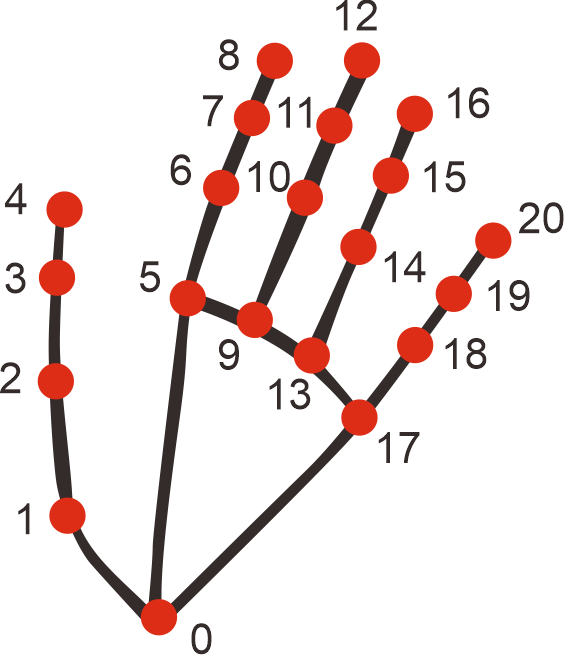
\includegraphics[scale=1]{gambar/mediapipe_hand_landmark.png}
  \caption{Hand Landmarks}
  \label{fig:handlandmarks}
\end{figure}

\begin{longtable}{|c|c|}
  \caption{Keterangan Nama Setiap Titik \emph{Landmark}}
  \label{tb:keterangansetiaptitiklandmark}\\
  \hline
  \textbf{Nomor titik} & \textbf{Keterangan} \\
  \hline
  \endhead
  0   & Pergelangan tangan  \\
  1   & Karpal Jempol   \\
  2   & Metakarpal Jempol   \\
  3   & Inter Falang Jempol  \\
  4   & Tuberocity Jempol  \\
  5   & Metakarpal Telunjuk  \\
  6   & Proksimal Palang Telunjuk  \\
  7   & Distal Palang Telunjuk  \\
  8   & Tuberocity Telunjuk  \\
  9   & Metakarpal Jari Tengah  \\
  10  & Proksimal Palang Jari Tengah  \\
  11  & Distal Palang Jari Tengah  \\
  12  & Tuberocity Jari Tengah  \\
  13  & Metakarpal Jari Manis  \\
  14  & Proksimal Palang Jari Manis  \\
  15  & Distal Palang Jari Manis  \\
  16  & Tuberocity Jari Manis  \\
  17  & Metakarpal Kelingking  \\
  18  & Proksimal Palang Kelingking  \\
  19  & Distal Palang Kelingking  \\
  20  & Tuberocity Kelingking  \\
  \hline
\end{longtable}

Dalam proses deteksi pose tangan ini, penulis menggunakan bantuan dari \emph{\emph{library} MediaPipe}. MediaPipe adalah kerangka kerja yang memungkinkan untuk membuat \emph{landmark}, atau titik-titik bagian dari kerangka anggota tubuh. Semua titik koordinat dinormalisasi tiga dimensi. MediaPipe menggunakan model \emph{landmark} pose, wajah dan tangan, namun yang digunakan pada penelitian ini hanyalah pada bagian tangan yang dimana terdapat 21 \emph{landmark} dalam tiap \emph{frame} sehingga menghasilkan citra kerangka tangan seperti yang ditunjukan pada Gambar \ref{fig:handlandmarks}. Setiap titik dalam kerangka tersebut merupakan representasi dari setiap bagian anatomi kerangka tangan. Daftar nama bagian dari setiap titik \emph{landmark} dapat dilihat pada Tabel \ref{tb:keterangansetiaptitiklandmark}. Dengan menggunakan \emph{\emph{library}} ini dapat langsung menghasilkan prediksi koordinat. Tiap \emph{landmark} yang ada memiliki koordinat x, y, dan z. Dimana untuk nilai x dan y dinormalisasi menjadi lebar dan tinggi dari gambar input yang diterima. Sedangkan z merepresentasikan nilai kedalaman \emph{landmark}, yang nilainya semakin kecil apabila tangan semakin mendekati kamera \parencite{Indriani2021}.

\subsection{Kontrol Microsoft PowerPoint}
Microsoft Office PowerPoint merupakan sebuah aplikasi komputer untuk presentasi yang dikembangkan oleh Microsoft di dalam paket aplikasi kantoran mereka yaitu Microsoft Office \parencite{Poerwanti2018}. PowerPoint pada awalnya dirancang untuk menyediakan visual untuk presentasi kelompok dalam organisasi bisnis. Namun, kemudian berkembang pesat ke sektor lainnya, baik dalam bisnis maupun di luarnya. Didalamnya terdapat berbagai fitur yang menunjang presentasi seperti navigasi berpindah \emph{slide}, \emph{pen tool} untuk mencoret-coret \emph{slide} beserta \emph{erase} untuk dapat menghapusnya. \emph{Pointer} untuk melakukan \emph{highlight} pada bagian tertentu. Hingga fitur \emph{zoom} untuk memperbesar bagian visual tertentu pada presentasi.

Fitur-fitur tersebut, dapat diakses salah satunya dengan menggunakan \emph{library} bernama \emph{pywin32}. \emph{Pywin32} adalah \emph{library} ekstensi \emph{python} untuk \emph{Windows} yang memungkinkan menggunakan fitur \emph{Aplication Programming Interface (API) Win32} di\emph{python}. Melalui \emph{library} ini, penggunaan fitur dalam PowerPoint bisa diakses melalui \emph{property} ataupun \emph{method} yang ada dalam object yang diinginkan. Tersedia juga dokumentasi untuk objek apa saja beserta \emph{property} dan \emph{method}-nya yang dapat diakses. Selain menggunakan \emph{library} ini, terdapat cara lain yaitu menggunakan \emph{library} yang berfungsi untuk menjalankan fungsi-fungsi yang ada pada \emph{keyboard}. Dikarenakan adanya keuntungan dalam menggunakan PowerPoint dimana tersedia opsi untuk mengakses fitur-fitur yang ada menggunakan shortcut tertentu pada \emph{keyboard}, maka dapat digunakan \emph{library} bernama \emph{pyautogui}. Dengan menggunakan kedua cara tersebut, membuat proses menghubungkan program \emph{python} yang dibuat bisa terhubung dengan aplikasi Microsoft PowerPoint.  

% MediaPipe dirancang untuk praktisi pembelajaran mesin (ML), termasuk peneliti, mahasiswa, dan pengembang perangkat lunak, yang mengimplementasikan aplikasi ML siap produksi,
% menerbitkan kode yang menyertai pekerjaan penelitian, dan membangun prototipe teknologi. Kasus penggunaan utama untuk MediaPipe adalah pembuatan prototipe cepat dari saluran persepsi dengan inferensi model dan komponen dapat digunakan kembali lainnya. MediaPipe juga memfasilitasi penerapan teknologi persepsi ke dalam deGambar 1: Deteksi objek menggunakan MediaPipe. Kotak transparan mewakili simpul perhitungan (kalkulator) dalam grafik MediaPipe, kotak padat mewakili input/output eksternal ke grafik, dan garis yang memasuki bagian atas dan keluar dari bagian bawah node masing-masing mewakili aliran input dan output. Port di sebelah kiri beberapa node menunjukkan paket sisi input. Lihat Bagian 6.1 untuk detailnya. mos dan aplikasi pada berbagai platform perangkat keras yang berbeda. MediaPipe memungkinkan peningkatan bertahap pada pipa persepsi melalui konfigurasinya yang kaya bahasa dan alat evaluasi.

% Memodifikasi aplikasi persepsi untuk memasukkan langkah-langkah pemrosesan tambahan atau model inferensi bisa jadi sulit, karena kopling yang berlebihan antara langkah-langkah. Selain itu, mengembangkan aplikasi yang sama untuk platform yang berbeda membutuhkan waktu mengkonsumsi dan biasanya melibatkan pengoptimalan inferensi dan memproses langkah-langkah agar berjalan dengan benar dan efisien pada target perangkat.

% MediaPipe mengatasi tantangan ini dengan mengabstraksi dan
% menghubungkan model persepsi individu menjadi dapat dipertahankan jalur pipa. Semua langkah yang diperlukan untuk menyimpulkan dari data sensorik dan mendapatkan hasil yang dirasakan ditentukan dalam konfigurasi pipa. Sangat mudah untuk menggunakan kembali komponen MediaPipe di pipeline yang berbeda di seluruh aplikasi yang berurutan karena komponen ini memiliki orientasi antarmuka yang sama sekitar data deret waktu. Setiap pipa kemudian dapat dijalankan dengan perilaku yang sama pada berbagai platform, memungkinkan praktisi untuk mengembangkan aplikasi pada workstation, dan lalu terapkan di seluler, misalnya. MediaPipe terdiri dari tiga bagian utama: (a) kerangka kerja untuk inferensi dari data sensorik, (b) seperangkat alat untuk evaluasi kinerja, dan (c) kumpulan inferensi yang dapat digunakan kembali dan komponen pemrosesan yang disebut kalkulator. Kami menjelaskan kerangka kerja di Bagian 3 dan 4, dan seperangkat alat di Bagian 5 Kami juga menyajikan contoh persepsi MediaPipe aplikasi di Bagian 6 \parencite{CamilloLugaresi}. 

\subsection{Convolutional Neural Network}

% \begin{figure} [ht] \centering  
%   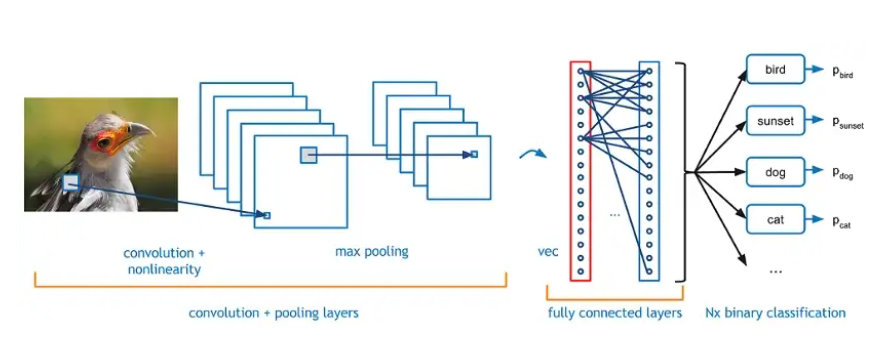
\includegraphics[scale=0.75]{gambar/teori-dasar-cnn.png}
%   \caption{Convolutional Neural Networks}
%   \label{fig:convolutionalneuralnetworks}
%   \parencite{CNN}
% \end{figure}

\emph{Convolutional Neural Network} atau disingkat menjadi CNN merupakan jenis \emph{neural network} yang digunakan dalam memproses data dua dimensi. Penggunaan nama \emph{Convolutional Neural Network} digunakan, karena terdapat operasi konvolusi yang terjadi didalamnya. Proses operasi konvolusi ini, membuat CNN hanya dapat digunakan pada data yang memiliki struktur dua dimensi seperti citra \parencite{IWayan2016}. Seperti jenis \emph{neural network} lainnya, dalam CNN terdapat \emph{hidden layer}. Namun, belum ada panduan yang betul-betul solid dalam menentukan jumlah \emph{hidden layer} pada sebuah arsitektur model CNN \parencite{MBernico}. Dalam \emph{hidden layer} CNN sendiri, terdapat tiga jenis lapisan utama yaitu :

\begin{enumerate}[nolistsep]
  \item Convolution Layer
  \item Pooling Layer
  \item Fully-connected Layer
\end{enumerate}

\subsubsection{Convolution Layer}

\begin{figure} [ht] \centering  
  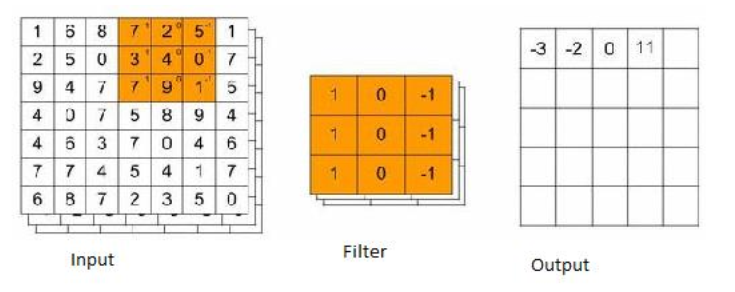
\includegraphics[scale=1]{gambar/convolution-operation.png}
  \caption{Ilustrasi Operasi Konvolusi}
  \label{fig:Ilustrasi Operasi Konvolusi}
  \parencite{MaxPoolingLayer}
\end{figure}

Pada bagian \emph{layer} ini, sebagian besar komputasi terjadi. Hal ini terjadi karena citra input diproses dengan operasi konvolusi dalam rangka menghasilkan filter citra yang berbeda-beda. Ada tiga komponen penting dalam \emph{layer} ini, yaitu input data, \emph{filter/kernel}, dan \emph{feature map}. Sebagai contoh, Input data yang diberikan dapat memiliki tiga dimensi. Tiga dimensi ini adalah lebar, tinggi, dan kanal. Perlu diketahui juga, bahwa pendekatan deep learning yang digunakan CNN merupakan \emph{supervised learning}. \emph{Supervised learning} adalah teknik pembelajaran menggunakan input dataset yang berlabel \parencite{MdZahangir}. Kemudian, untuk \emph{filter/kernel} memiliki tugas untuk bergerak melintasi citra dan melakukan operasi "dot" antara input citra dengan matriks dari filter. Hasil operasi ini adalah \emph{output} yang biasa disebut dengan \emph{feature map}. Keseluruhan proses inilah yang dikenal dengan istilah konvolusi. Ilustrasi proses operasi konvolusi ini dapat dilihat pada gambar \ref{fig:Ilustrasi Operasi Konvolusi}.


Pada Gambar \ref{fig:Ilustrasi Operasi Konvolusi} dapat diketahui bahwa filter bisa berjumlah banyak dan memiliki bentuk berupa matriks. Nilai pada filter tersebut adalah \emph{weight} yang dapat diperbarui nilainya saat proses pelatihan. Dalam \emph{layer} ini terdapat \emph{hyperparameter} yang bisa diatur. Berikut beberapa diantaranya :

\begin{enumerate}[nolistsep]
  \item Jumlah filter. Banyaknya filter yang digunakan berpengaruh terhadap banyaknya kanal pada \emph{feature map}. Jadi, jika terdapat dua filter yang berbeda misalnya, maka \emph{feature map} yang dihasilkan juga dua dengan nilai yang berbeda.
  \item \emph{Stride}. \emph{Stride} merupakan besarnya jarak perpindahan yang dilalui filter saat melintasi citra saat proses konvolusi. Hal ini mengakibatkan apabila semakin besar nilai \emph{stride}, maka ukuran \emph{output} yang dihasilkan semakin kecil. 
  \item \emph{Padding}. \emph{Padding} adalah bagian yang ditambahkan pada elemen terluar citra. Umumnya, nilai yang ditambahkan adalah 0 dengan ukuran yanng berbeda-beda. Terdapat tiga jenis \emph{padding} yaitu \emph{valid padding, same padding, dan full padding}. 
\end{enumerate}   

\subsubsection{\emph{Pooling Layer}}

\begin{figure} [ht] \centering  
  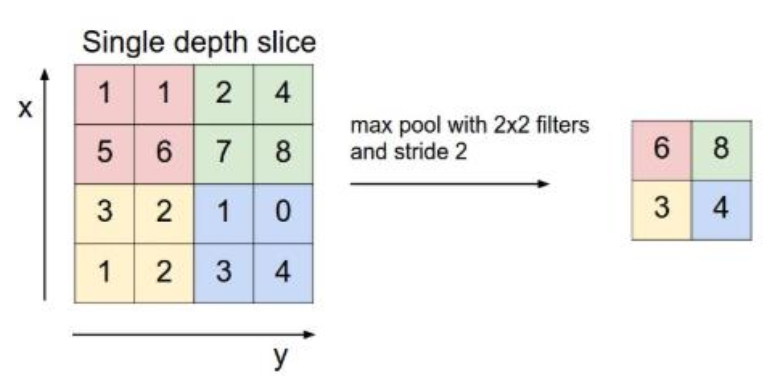
\includegraphics[scale=0.85]{gambar/max-pooling-layer.png}
  \caption{Ilustrasi Max Pooling Layer}
  \label{fig:Ilustrasi Max Pooling Layer}
  \parencite{MaxPoolingLayer}
\end{figure}

\emph{Pooling layer} adalah bagian \emph{layer} yang memiliki fungsi untuk \emph{downsampling}. \emph{Downsampling} adalah pengurangan ukuran dimensi dan jumlah parameter. Hal ini dilakukan dengan tujuan mengurangi tingkat kompleksitas untuk \emph{layer} selanjutnya karena proses ini membuat resolusi dari nilai matriks suatu citra menjadi lebih berkurang. Selain itu, \emph{pooling layer} juga berfungsi untuk mengekstraksi fitur dominan. Umumnya, Ada dua jenis \emph{pooling} yang dapat digunakan yaitu \emph{max pooling} dan \emph{average pooling}. \emph{Max pooling} mengambil nilai maksimum dari citra yang ada dalam suatu \emph{kernel}. \emph{Average pooling} mengambil nilai rata-rata dari citra yang dalam suatu \emph{kernel}. 

Sebagai contoh, untuk \emph{max pooling} dapat dilihat dalam gambar \ref{fig:Ilustrasi Max Pooling Layer}. Pada matriks tersebut, ukurannya dibagi tiap kotak 2x2. Tiap bagian kotak tersebut, dicari nilai paling besarnya dan dijadikan \emph{output} dari nilai matriks yang baru. Begitu juga dengan \emph{average pooling}, prosesnya mirip namun yang membedakan hanya pada nilai yang diambil dari bagian matriks yang dipotongnya. \emph{Output} nilai matriks yang baru dalam \emph{average pooling} didapatkan dari hasil rata-rata dalam kotak matriks yang dibagi. 

\subsubsection{Fully Connected Layer}

\begin{figure} [ht] \centering  
  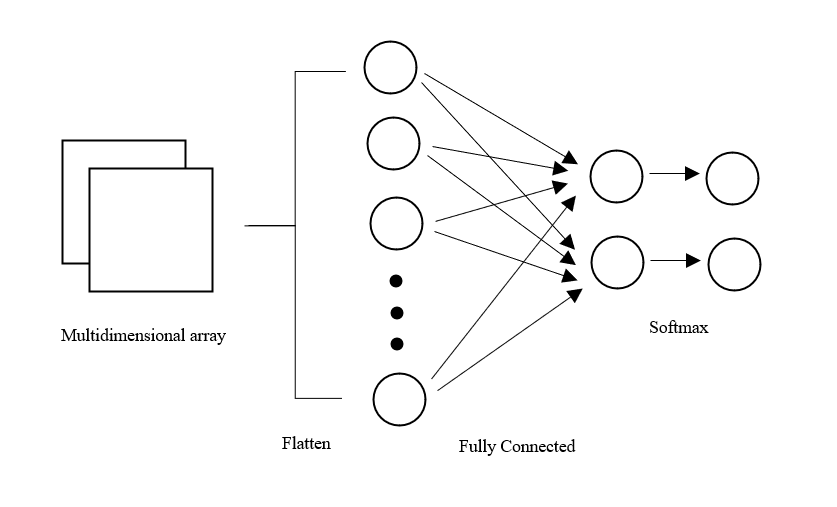
\includegraphics[scale=0.7]{gambar/fully-connected.png}
  \caption{Ilustrasi Fully connected}
  \label{fig:Ilustrasi Fully connected}
\end{figure}

Dalam Gambar \ref{fig:Ilustrasi Fully connected} terdapat sebuah ilustrasi mengenai serangkaian proses yang terjadi dalam layer ini. Proses awalnya dimulai dari hasil \emph{feature map} pada convolution dan pooling \emph{layer} yang memiliki bentuk \emph{multidimensional array}. Bentuk ini perlu dilakukan reshape menjadi sebuah vektor. Tujuannya, agar dapat menjadi input dari \emph{fully connected layer}. Vektor ini juga dapat disebut sebagai \emph{flatten}, dimana hasilnya terhubung dengan beberapa neuron. Setiap koneksi pada neuron tersebut memiliki \emph{weights} yang terkait. Besaran nilai \emph{weights} ini sendiri didapatkan saat proses \emph{training} model. 

Saat proses sudah mencapai dalam neuron yang mengandung \emph{weights} tersebut, diterapkanlah fungsi aktivasi. Fungsi dari diterapkannya fungsi aktivasi ini untuk menghitung probabilitas dalam setiap kelas yang ada pada model. Dalam melakukan klasifikasi, fungsi aktivasi yang digunakan biasanya adalah \emph{softmax}. Hasil akhir dari \emph{softmax} merupakan nilai probabilitas dengan rentang dari 0 sampai 1. Dari nilai probablitas ini biasanya dipilih nilai yang paling besar diantara yang lain dengan juga menerapkan \emph{threshold} yang menjadi nilai minimum untuk menyatak suatu citra masuk dalam kelas tertentu.

\subsection{\emph{Confusion Matrix}}

\emph{Confusion matrix} adalah parameter yang digunakan untuk mengukur kinerja model klasifikasi. Salah satu fungsi utama dari \emph{confusion matrix} adalah untuk mengetahui distribusi atau persebaran dari hasil klasifikasi. Dapat diketahui juga berapa jumlah data yang terdeteksi dalam kelas yang benar atau salah. \emph{Confusion matrix} dapat diterapkan untuk klasifikasi biner dan klasifikasi multi-class. Terdapat beberapa istilah dalam Confusion matrix yaitu TP, TN, FP, dan FN. Namun, penggunaan istilah yang paling sering digunakan dalam menentukan akurasi adalah TP. Berikut adalah penjelasan tiap istilah tersebut \parencite{MohammadReza}.

\begin{enumerate}[nolistsep]
  \item True Positive (TP)
  TP menunjukkan jumlah sampel positif yang diprediksi secara akurat. Contohnya pada klasifikasi suatu gambar. sistem memprediksi bahwa gambar termasuk kelas A dan memang benar gambar tersebut termasuk kelas A.
  \item True Negative (TN)
  TN menunjukkan jumlah sampel negatif yang diprediksi secara akurat. Contohnya pada klasifikasi suatu gambar. sistem memprediksi bahwa gambar tidak termasuk kelas A dan memang benar gambar tersebut tidak termasuk kelas A.
  \item False Positive (FP)
  FP menunjukkan jumlah sampel yang sebenarnya negatif tetapi diprediksi positif. Contohnya pada klasifikasi suatu gambar, sistem memprediksi bahwa gambar termasuk kelas A, namun ternyata gambar tersebut tidak termasuk kelas A. Itu artinya prediksi tersebut salah.
  \item False Negative (FN)
  FN menunjukkan jumlah sampel yang sebenarnya positif tetapi diprediksi negatif. Contohnya pada klasifikasi suatu gambar, sistem memprediksi bahwa gambar tidak termasuk kelas A. namun ternyata gambar tersebut termasuk kelas A. Itu artinya prediksi tersebut salah.
\end{enumerate}   

Hasil dari \emph{confusion matrix} ini dapat ditunjukkan  kedalam beberapa metrik untuk mengevaluasi klasifikasi yaitu \emph{precision, recall,} dan \emph{f1 score}. \emph{Precision} adalah metrik yang digunakan untuk mengukur tingkat presisi hasil dari klasifikasi. Persamaan yang digunakan untuk mendapatkan nilai \emph{precision} dapat dilihat pada Rumus \ref{eq:rumus precision}.

\begin{equation}
  \label{eq:rumus precision}
  \emph{Precision} = \frac{TP}{TP+FP}
\end{equation}

Sedangkan, \emph{recall} merupakan metrik yang digunakan untuk mengetahui seberapa banyak objek yang dapat dideteksi oleh model. \emph{Recall} juga bisa disebut \emph{sensitivity} karena menggambarkan tingkat sensitifitas model saat mendeteksi. Melalui \emph{recall} dapat diketahui seberapa besar peluang kasus kategori positif dapat tepat diprediksi secara positif juga. Nilai dari \emph{recall} dapat dicari menggunakan Persamaan \ref{eq:rumus recall}.

\begin{equation}
  \label{eq:rumus recall}
  \emph{Recall} = \frac{TP}{TP+FN}
\end{equation}

Terakhir terdapat \emph{f1 score}, yaitu metrik yang menunjukkan nilai perbandingan antara rata-rata dari nilai \emph{precision} dengan nilai \emph{recall}. Secara sederhana, dikarenakan \emph{f1 score} memasukkan nilai \emph{precision} dan \emph{recall} kedalam perhitungannya, maka \emph{f1 score} membuat nilai \emph{False Positive} dan \emph{False Negative} juga masuk kedalam penilaiannya. Sehingga, metrik \emph{f1 score} juga menggambarkan resiko kesalahan dari \emph{False Positive} dan \emph{False Negative}. Rumus menghitung \emph{f1 score} sendiri dapat dilihat pada Persamaan \ref{eq:rumus f1score}

% Penggunaan \emph{f1 score} dinilai lebih tepat sebagai acuan performa model dibandingkan dengan akurasi apabila dalam kondisi dimana dataset menunjukkan jumlah data antara \emph{False Negatif} dengan \emph{False Positif} yang tidak mendekati. Apabila jumlahnya mendekati, maka dapat menggunakan akurasi saja sebagai acuan performa model. 

\begin{equation}
  \label{eq:rumus f1score}
  \emph{F1 Score} = \frac{2 \times Precision \times Recall}{Precision + Recall}
\end{equation}

% Representasi dasar \emph{confusion matrix} juga dapat dilihat pada tabel, dimana istilah TP, TN, FP, dan FN dapat divisualisasikan menjadi data berbentuk tabel.

% \begin{longtable}{|c|c|c|}
%   \caption{Representasi Dasar \emph{Confusion Matrix}}
%   \label{tb:Representasi Dasar Confusion Matrix}\\
%   \hline
%   \textbf{} & \textbf{Hasil Prediksi 0} & \textbf{Hasil Prediksi 1} \\
%   \hline
%   Realita 0   &  True Negative    & False Positive  \\
%   Realita 1   &  False Negative   & True Positif  \\
%   \hline
% \end{longtable}

% Kemudian menjadi persamaan seperti pada persamaan \ref{eq:hukumpertamanewton}.

% % Contoh pembuatan persamaan

